%
% teil1.tex -- Beispiel-File für das Paper
%
% (c) 2020 Prof Dr Andreas Müller, Hochschule Rapperswil
%
% !TEX root = ../../buch.tex
% !TEX encoding = UTF-8
%
\section{Grundbegriffe der Baustatik}
\label{balken:section:teil1}
\begin{description}
\item[\textbf{Balken}] Ein «Balken» ist ein langer, schmaler Körper, der hauptsächlich Querkräften sowie Biegebelastungen ausgesetzt ist.
Balken können unterschiedliche Formen annehmen.
\item[\textbf{Balkengleichung}] Die Balkengleichung (auch als Euler-Bernoulli-Balkengleichung (EBB) bekannt) beschreibt das Biegeverhalten eines Balkens unter der Einwirkung von Querkräften und / oder Momenten.
Dieses Biegeverhaltens wird grafisch durch eine Biegelinie illustriert. \ref{balken:Biegelinie}
\begin{equation}
	\frac{d^2}{{dx}^2}\left(EI\frac{d^2y}{{dx}^2}\right)
	=-M(x)
\end{equation}
$E$ = Elastizitätsmodul des Balkenmaterials

$I$ = Flächenträgheitsmoment des Balkenquerschnitts

$y(x)$ = vertikale Verschiebung des Balkens als Funktion der horizontalen Position x

$M(x)$ = Biegemoment entlang des Balkens

Diese Gleichung beschreibt die Beziehung zwischen der Biegemomentenverteilung entlang des Balkens M(x) und der daraus resultierende Verformung y(x).
\item[\textbf{Biegelinie $u(x)$}] Eine visuelle Darstellung, die das Verhalten eines Balkens unter Einwirkung von Querkräften und/oder Momenten veranschaulicht und die Krümmung des Balkens entlang seiner Länge darstellt. \ref{balken:Biegelinie}
\begin{figure} [h]
	\centering
	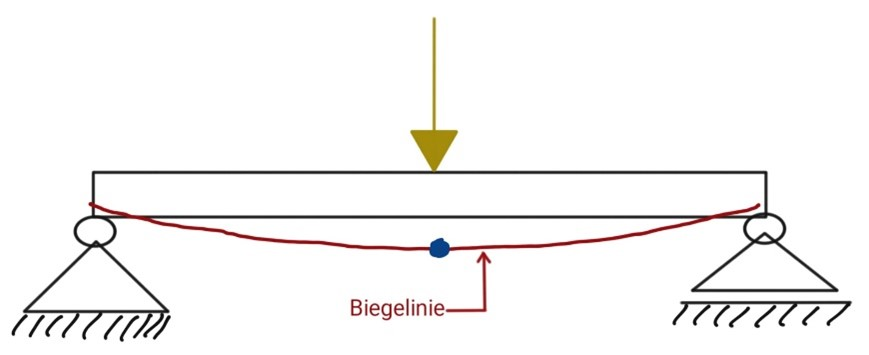
\includegraphics[width=0.8\textwidth]{papers/balken/images/teil1/Biegelinie1.jpg}
	\caption{Abbildung der Biegelinie aufgrund einer Einzellast}
	\label{fig:Abbildung der Biegelinie aufgrund einer Einzellast}
\end{figure}
\item[\textbf{Biegemoment ($M$)}] Das Biegemoment, auch Schnittmoment genannt, ist eine Beanspruchung, bei dem ein Drehmoment erzeugt wird.
Diese Beanspruchung kann entweder durch eine vertikale Kraft mit einem Hebelarm ausgelöst werden
\begin{equation}
	M=
	F\cdot\ s
\end{equation}
oder durch ein bereits vorhandenes Drehmoment selbst.
Biegemomente entstehen, wenn eine Kraft auf einen Körper einwirkt und eine Biegung oder Drehung auszulösen versucht.
\begin{figure} [h]
	\centering
	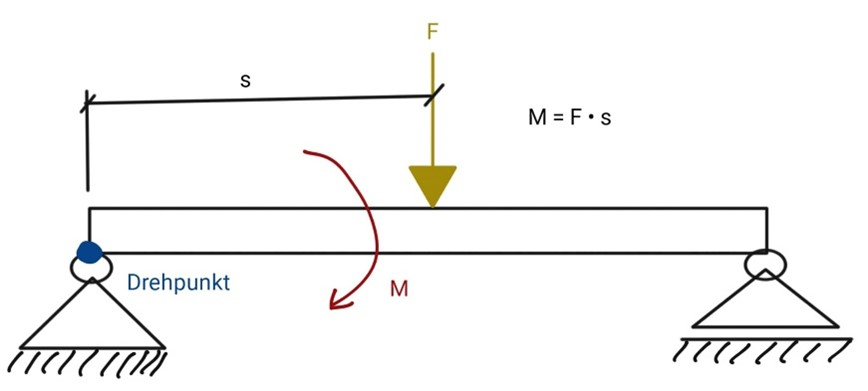
\includegraphics[width=0.8\textwidth]{papers/balken/images/teil1/Biegemoment.jpg}
	\caption{Die Abbildung zeigt einen Balken, der von einer einzigen Last belastet wird, was zu auftretenden Momenten führt.}
	\label{fig:Die Abbildung zeigt einen Balken, der von einer einzigen Last belastet wird, was zu auftretenden Momenten führt.}
\end{figure}
\item[\textbf{Biegesteifigkeit ($σ_B$, $R$)}] Die Biegesteifigkeit besagt wie widerstandsfähig ein Material und Form gegen eine Biegebeanspruchung ist.
Sie beschreibt die Fähigkeit eines Balkens, sich unter äusserliche Einwirkung eines Biegemomentes zu verformen.
\begin{equation}
\sigma_{B,R}=E
\left(x\right)\cdot\ I\left(x\right)=
\frac{M(x)}{W(x)}
\end{equation}
$E(x)$ = Elastizitätsmodul

$I(x)$ = Flächenträgheitsmoment

$M(x)$ = Moment 

$W(x)$ = Widerstandsmoment

\item[\textbf{E-Modul ($E$)}] Das E-Modul ist eine Materialkonstante, welches die Steifigkeit eines Materials beschreibt.
Er gibt an, wie viel Spannung ein Material aushalten kann, bis das Material eine bestimmte Dehnung erfährt. \ref{balken:Elastizitätsmodul}
Der E-Modul wird definiert als
\begin{equation}
E=
\frac{\sigma}{\varepsilon}
\end{equation}
$σ$ = Spannung

$ε$ = Dehnung

\item[\textbf{Festlager}] Ein Festlager ist ein Lager, das fähig ist, Kräfte in horizontaler und vertikaler Rich-tung aufzunehmen, jedoch keine Momente aufnehmen kann.
Aufgrund dieser Eigenschaften werden Festlager als 2-wertige Auflager bezeich-net, da sie zwei Auflagerreaktionen haben (Querkräfte und Horizontalkräfte) und nur einen Freiheitsgrad (Momente) besitzen.
\begin{figure} [h]
	\centering
	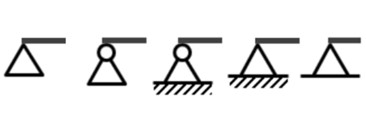
\includegraphics[width=0.8\textwidth]{papers/balken/images/teil1/Festlager.jpg}
	\caption{Die Abbildung zeigt verschiedene Darstellungsweisen eines Festlagers in der Baustatik.}
	\label{fig:Die Abbildung zeigt verschiedene Darstellungsweisen eines Festlagers in der Baustatik.}
\end{figure}
\item[\textbf{Flächenträgheitsmoment ($I$)}] Das Flächenträgheitsmoment gibt die Trägheit eines Körpers an gegenüber einer Änderung seiner Drehbewegung.
Anders ausgedrückt gibt es an, wie widerstandsfähig ein Bauteil gegen Biegung ist.
Diese Trägheit wird ausschliesslich durch die Form des Körpers bestimmt, weshalb das Flächenträgheitsmoment von der Geometrie des Querschnittes abhängt.
\item[\textbf{Lasten}] Lasten sind Kräfte oder Belastungen, die auf einen Körper bzw. statischen System wirken.
Sie können aufgrund von Gewichtskräfte, externe Kräfte, thermische Belastungen und vieles mehr auftreten.
Lasten gibt es in vier verschiedene Arten.
\begin{figure} [h]
	\centering
	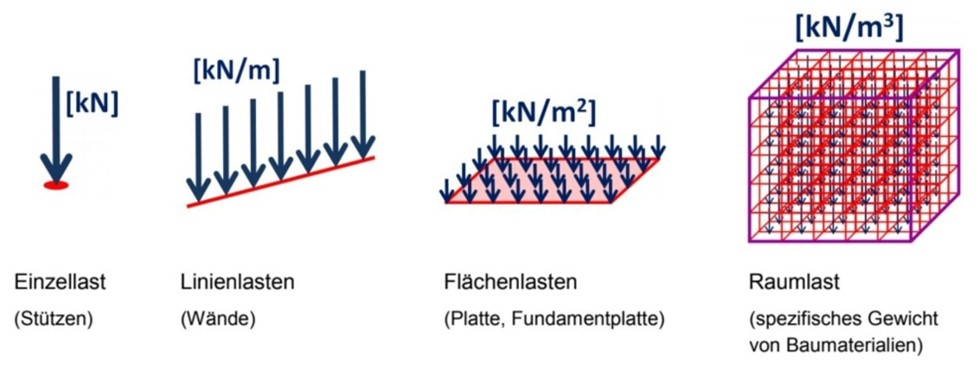
\includegraphics[width=0.8\textwidth]{papers/balken/images/teil1/Lasten.jpg}
	\caption{Die Abbildung zeigt verschiedene Lasttypen, die in der Baustatik vorkommen.}
	\label{fig:Die Abbildung zeigt verschiedene Lasttypen, die in der Baustatik vorkommen.}
\end{figure}
\item[\textbf{Loslager}] Loslager besitzen die Fähigkeit Querkräfte aufzunehmen und werden deshalb als statisch 1-wertige Auflagern genannt.
Da sie Horizontalkräfte und Momenten nicht aufnehmen können, besitzen sie zwei Freiheitsgrade.
\begin{figure} [h]
	\centering
	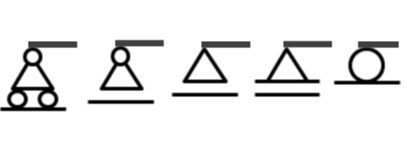
\includegraphics[width=0.8\textwidth]{papers/balken/images/teil1/Loslager.jpg}
	\caption{Das Bild zeigt unterschiedliche Arten, ein Loslager in der Baustatik darzustellen.}
	\label{fig:Das Bild zeigt unterschiedliche Arten, ein Loslager in der Baustatik darzustellen.}
\end{figure}
\begin{figure} [h]
\centering
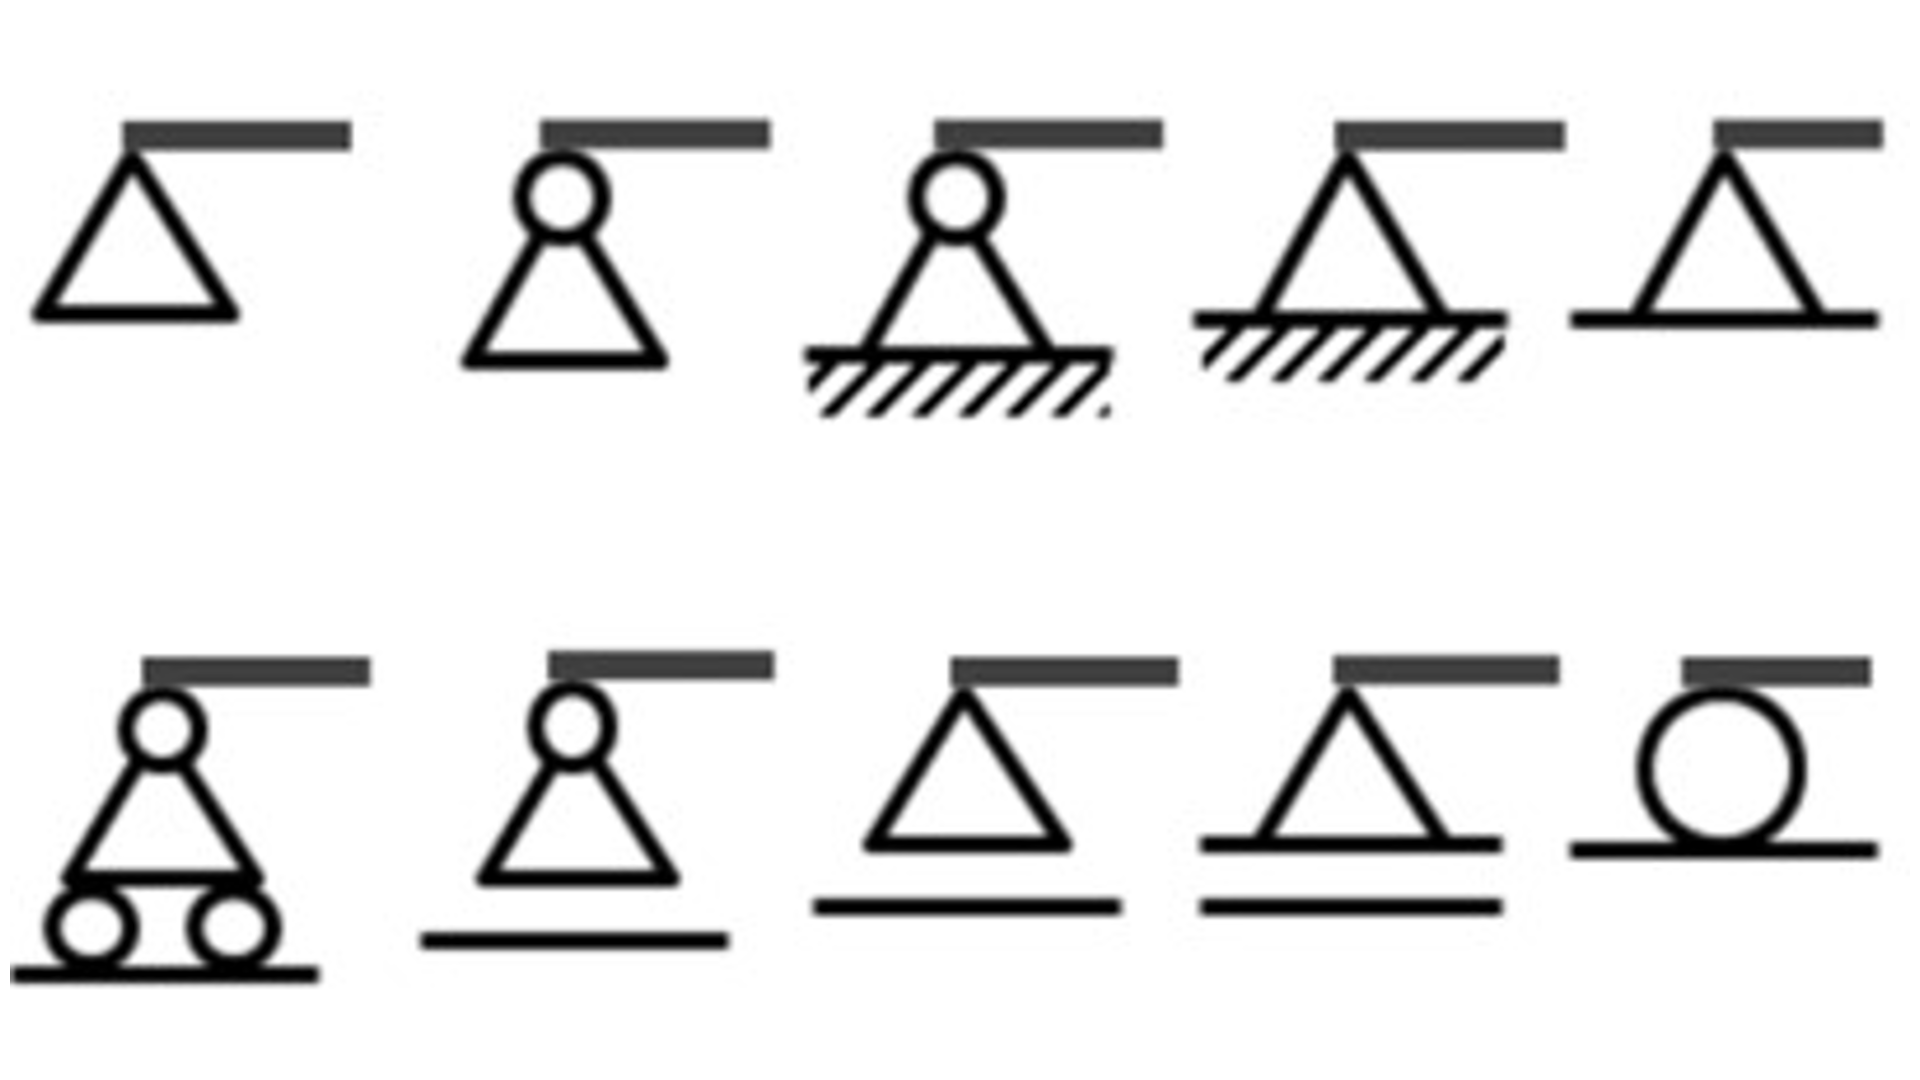
\includegraphics[width=0.8\textwidth]{papers/balken/images/teil1/Gegenueberstellung.png}
\caption{Diese Abbildung zeigt die unterschiedlichen Darstellungsweisen von Festlagern und Loslagern. Oben das Festlager abgebildetet und unten das Loslager.}
\label{fig:Diese Abbildung zeigt die unterschiedlichen Darstellungsweisen von Festlagern und Loslagern. Oben das Festlager abgebildetet und unten das Loslager.}
\end{figure}
\item[\textbf{Nulllinie}] Die Nulllinie ist eine Referenzlinie, von der Berechnungen durchgeführt werden. Sie dient als Bezugspunkt für Abständen und Winkeln.
Die Nulllinie ist dort wo die Fasern des Baumaterials neutral, sprich unbelastet sind.
Bei einachsigen Beanspruchungen liegt die Nulllinie typischerweise in der Mitte des Querschnitts.
Bei schräger Biegung verläuft die Nulllinie jedoch schräg durch den Querschnitt.
\item[\textbf{Querkraft ($Q$)}] Querkräfte sind Kräfte, die senkrecht zur Längsrichtung eines Bauteils wirken.
Sie üben Druck- und Zugkräfte seitlich auf den Bauteil aus, was zu Biegungen führen kann.
\item[\textbf{Widerstandsmoment ($W$)}] Das Widerstandsmoment
\begin{equation}
W=I/c
\end{equation}
$W$ = Widerstandsmoment

$I$ = Flächenträgheitsmoment

$c$ = Abstand des äusseren Fasermittelpunkts zu der neutralen Faser

kann mithilfe des Flächenträgheitsmoments berechnet werden.
Es gibt an, welchen Widerstand ein belastetes Bauteil den inneren Spannungen entgegensetzt.
\end{description}
\subsection{Einführung in die Balkengleichung}
Wirken Lasten auf einen Balken, so führt es zu einer Verformung der Balken aufgrund von auftretenden Momenten um die $y$-Achse.
Die Balkentheorie analysiert diese Verformungen unter verschiedenen Lastszenarien und bestimmt dadurch die Biegelinie des Balkens, welche den Verlauf der Verformung entlang seiner Länge beschreibt.
Wir wollen nun die Balkengleichung der Biegelinie $u(x)$ herleiten. \ref{balken:Balkentheorie}

Wir betrachten einen schmalen Balken, welche seine Länge $L$ entlang der $x$-Achse verläuft.
Allfällige Momente wirken um den $y$-Achse im Uhrzeigersinn und erzeugen eine positive Biegelinie u(x) mit der Öffnung gegen oben.
D.h. $u(x) > 0$.
Dabei verwenden wir die Euler-Bernoulli-Balkengleichung (EBB), die gültig ist, wenn reine Biegung so-wie Querkraftbiegungen auftreten.
Für die EBB werden ausschliesslich Querschnitte betrachtet, die lotrecht zur Nulllinie liegen (im unbelasteten Zustand). \ref{balken:Biegelinie}